\documentclass[a4paper,12pt]{extarticle}
\usepackage[utf8x]{inputenc}
\usepackage[T1,T2A]{fontenc}
\usepackage[russian]{babel}
\usepackage{indentfirst}
\usepackage{listings}
\usepackage{color}
\usepackage{here}
\usepackage{array}
\usepackage{multirow}
\usepackage{graphicx}
\usepackage[hidelinks]{hyperref}

\usepackage{caption}
\renewcommand{\lstlistingname}{Программа} % заголовок листингов кода

\bibliographystyle{ugost2008ls}

\lstset{ %
extendedchars=\true,
keepspaces=true,
language=SQL,						% choose the language of the code
basicstyle=\footnotesize,		% the size of the fonts that are used for the code
numbers=left,					% where to put the line-numbers
numberstyle=\footnotesize,		% the size of the fonts that are used for the line-numbers
stepnumber=1,					% the step between two line-numbers. If it is 1 each line will be numbered
numbersep=5pt,					% how far the line-numbers are from the code
backgroundcolor=\color{white},	% choose the background color. You must add \usepackage{color}
showspaces=false				% show spaces adding particular underscores
showstringspaces=false,			% underline spaces within strings
showtabs=false,					% show tabs within strings adding particular underscores
frame=single,           		% adds a frame around the code
tabsize=2,						% sets default tabsize to 2 spaces
captionpos=t,					% sets the caption-position to top
breaklines=true,				% sets automatic line breaking
breakatwhitespace=false,		% sets if automatic breaks should only happen at whitespace
escapeinside={\%*}{*)},			% if you want to add a comment within your code
postbreak=\raisebox{0ex}[0ex][0ex]{\ensuremath{\color{red}\hookrightarrow\space}},
texcl=true,
inputpath=../src,                     % директория с листингами
}

\usepackage[left=2cm,right=2cm,
top=2cm,bottom=2cm,bindingoffset=0cm]{geometry}

%%Нумерация картинок по секциям
\let\counterwithin\relax
\let\counterwithout\relax
\usepackage{chngcntr}
\counterwithin{figure}{section}
\counterwithin{table}{section}

%%Точки нумерации заголовков
\usepackage{titlesec}
\titlelabel{\thetitle.\quad}
\usepackage[dotinlabels]{titletoc}

%%Оформления подписи рисунка
\addto\captionsrussian{\renewcommand{\figurename}{Рисунок}}
\captionsetup[figure]{labelsep = period}

%%Подпись таблицы
\DeclareCaptionFormat{hfillstart}{\hfill#1#2#3\par}
\captionsetup[table]{format=hfillstart,labelsep=newline,justification=centering,skip=-10pt,textfont=bf}


\begin{document}	% начало документа

% Титульная страница
\def\subjectName{Базы данных}
\def\titleName{Разработка структуры БД}
\def\workNumber{1}
\def\studentName{Еременко Д.Ю.}
\def\groupNumber{33531/2}
\def\teacherName{Мяснов А.В.}

\begin{titlepage}	% начало титульной страницы
	\begin{center}		% выравнивание по центру
		\large Санкт-Петербургский Политехнический Университет Петра Великого\\
 		\begin{center}
 		\underline{\hspace{30em}}
 		\end{center}
		\large Институт компьютерных наук и технологий \\
		\large Кафедра компьютерных систем и программных технологий\\[6cm]
		% название института, затем отступ 6см
		\huge \subjectName \\[0.5cm] % название работы, затем отступ 0,5см
		\large Отчет по лабораторной работе №\workNumber \\[0.1cm]
		\large Тема работы: "\titleName "\\[5cm]
	\end{center}
	\begin{flushright} % выравнивание по правому краю
				\large\textbf{Работу выполнил:}\\
				\large \studentName\\
				\large {Группа:} \groupNumber \\
				\large \textbf{Преподаватель:}\\
				\large \teacherName
	\end{flushright}	
	\vfill % заполнить всё доступное ниже пространство
	\begin{center}
	\large Санкт-Петербург\\
	\large \the\year % вывести дату
	\end{center} % закончить выравнивание по центру
\thispagestyle{empty} % не нумеровать страницу
\end{titlepage} % конец титульной страницы
\vfill % заполнить всё доступное ниже пространство

% Содержание
\renewcommand\contentsname{\centerline{Содержание}}
\tableofcontents
\newpage


\section{Цель работы}
Познакомиться с основами проектирования схемы БД, способами организации данных в SQL-БД.

\section{Программа работы}

\begin{enumerate}
\item Создать проект для работы на GitLab.
\item Выбрать задание (предметную область), описать набор данных и требований к хранимым данным в свободном формате в wiki своего проекта на GitLab.
\item Сформировать в свободном формате (предпочтительно в виде графической схемы) схему БД, соответствующую заданию. Должно получиться не менее 7 таблиц.
\item Согласовать с преподавателем схему БД. Обоснавать принятые решения и соответствие требованиям выбранного задания.
\item Выложить схему БД в свой проект на GitLab.
\item Продемонстрировать результаты преподавателю.
\end{enumerate}

\section{Ход выполнения работы}

\begin{enumerate}
\item Создание проекта на GitLab: \url{http://gitlab.icc.spbstu.ru/Eremenko/RDB};
\item Выбор предметной области: "Домашний Холодильник";
\item Формирование схемы БД средствами DataGrip : 8 таблиц;
\item Согласование схемы с преподавателем;
\item Внесение поправок;
\item Написание отчета;
\item Загрузка отчета на GitLab.
\end{enumerate}

\newpage
БД холодильника состоит из 8 таблиц:
\\\\-\textit{refregerator} хранит информацию о хранящихся в холодильнике продуктах: магазин, цена, скидка, день покупки, срок годности, количество;
\\\\-\textit{product} хранит информацию доступных для хранения в холодильнике продуктах: название, производитель, приоритет, состояния, тип продукта;
\\\\-\textit{recipe} хранит название блюда и способ его приготовления;
\\\\-\textit{recipe\_product} является соединительной таблицей со связью многие ко многим и хранит информацию о продуктах, необходимых для приготовления блюда;
\\\\-\textit{market\_name} содержит имена доступных магазинов;
\\\\-\textit{product\_type} содержит допустимые типы продуктов;
\\\\-\textit{cook\_condition} содержит допустимые состояния продуктов;
\\\\-\textit{way\_of\_cooking} содержит допустимые способы приготовления блюд;
\\\\




Схема показана на Рис. \ref{pic:db-schema}.

\begin{figure}[H]
	\begin{center}
		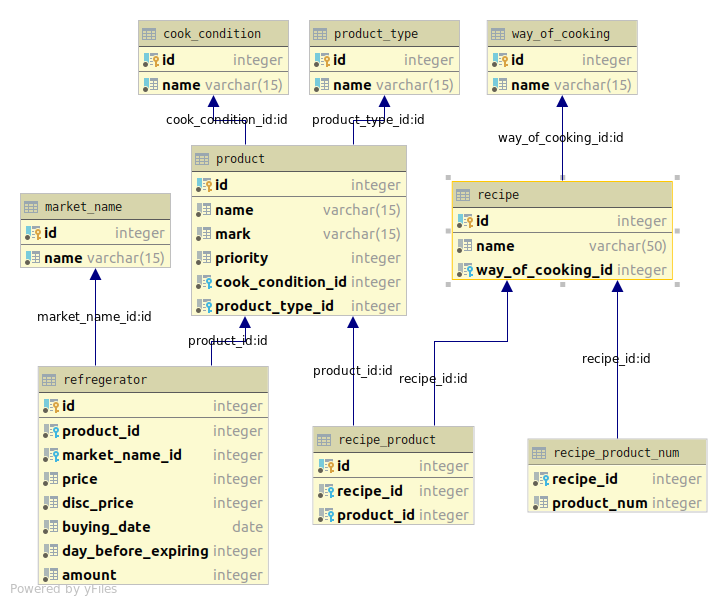
\includegraphics[scale=0.5]{refregerator.png}
		\caption{Модель} 
		\label{pic:db-schema} % название для ссылок внутри кода
	\end{center}
\end{figure}

\section{Выводы}

В данной работе была провередена подготовка таблиц для дальнейшей их реализации в базе данных PostgreSQL.

\end{document}
